\documentclass[12pt, a4paper]{article}
\usepackage[utf8]{inputenc}
\usepackage[T1]{fontenc}
\usepackage{graphicx}
\usepackage{hyperref}

\textwidth=170mm
\textheight=257mm
\oddsidemargin=0mm
\topmargin=0mm
\headheight=0mm
\headsep=0mm
\footskip=20mm
\graphicspath{ {./} }

\hypersetup{
    colorlinks=true,
    linkcolor=blue,
    urlcolor=blue,
}

\pagestyle{plain}

\begin{document}

% --- Title Page Setup ---
\begin{titlepage}
\centering
\vspace*{1cm}

% First report page image
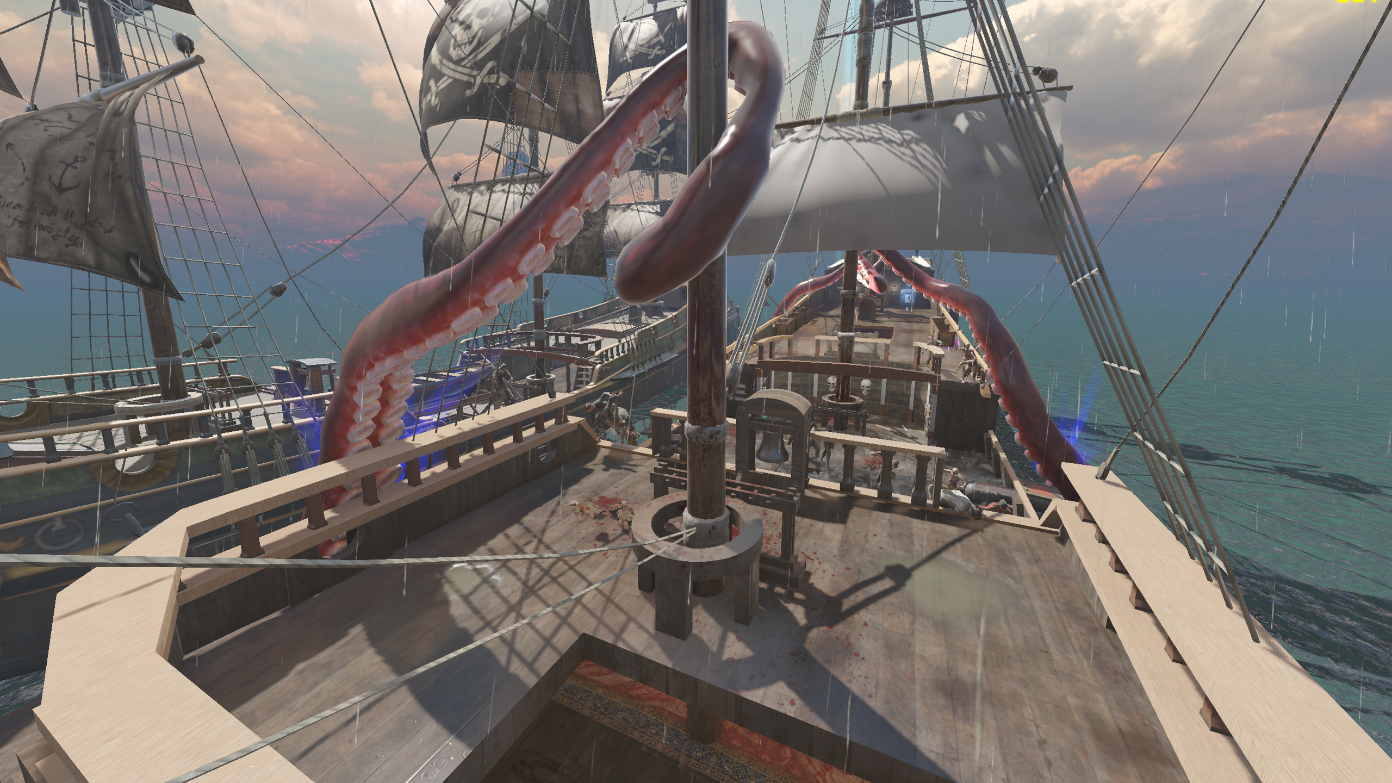
\includegraphics[width=0.9\textwidth]{AAST.png}
\vspace{1.5cm}

{\Large Bershama --- Egyptian Pharmaceutical Distribution Platform}\\
{\large Web Console --- Remediation Plan and Mobile App Phase 1 Submission}\\
\vspace{0.3cm}
{\large Software Engineering Course --- Project Submission Phase 1}\\
\vspace{2.5cm}

\begin{minipage}{0.7\textwidth}
\centering
\begin{tabular}{l l}
\multicolumn{2}{l}{\textbf{Source (GitHub):}} \\
\multicolumn{2}{l}{\url{https://github.com/lonelyb0y/bershama}} \\
\multicolumn{2}{l}{\textbf{Deployed:}} \\
\multicolumn{2}{l}{\url{https://pharmaflow-bay.vercel.app}} \\
\end{tabular}
\end{minipage}
\vspace{2cm}

\begin{minipage}{0.7\textwidth}
\centering
\begin{tabular}{l l}
\multicolumn{2}{l}{\textbf{Presented by:}} \\
1. Team Member One & ID --- \\
2. Team Member Two & ID --- \\
3. Team Member Three & ID --- \\
4. Team Member Four & ID --- \\
5. Team Member Five & ID --- \\
\end{tabular}
\end{minipage}
\vspace{2cm}

\begin{minipage}{0.7\textwidth}
\centering
\begin{tabular}{l}
\textbf{Presented to:} \\
Course Instructor \\
\end{tabular}
\end{minipage}
\vspace{3cm}

\vspace{1cm}

\end{titlepage}

\clearpage

% --- Content Start ---

\section{Introduction and System Overview}

The Bershama system is an Egyptian pharmaceutical distribution platform built as a web console (Next.js 16, App Router, next-intl, Supabase, Vercel free tier). The source code and all design assets are maintained on GitHub; this report pulls the system description, defect register, and remediation tasks from that repository rather than duplicating them inline.

\subsection{System Objective}

Bershama automates pharmaceutical stock distribution across hubs, pharmacies, distributors, and driver routes. Core capabilities include inventory catalogue management, batch/expiry tracking, requisition queues, delivery run planning and proof capture, cold-chain telemetry, an alert centre, role-based access control, and account settings. The system enforces tenant isolation through Supabase RLS and surfaces a single authenticated shell with navigation, console dock, and user cluster.

\subsection{Source Reference}

All implementation details---including the full defect register, ordered fix tasks, acceptance gates, and the master remediation prompt---are maintained in the GitHub repository:

\begin{itemize}
    \item Repository: \url{https://github.com/lonelyb0y/bershama}
    \item Remediation plan: \texttt{docs/superpowers/plans/2026-10-29-bershama-remediation.md}
    \item Copy-paste master prompt: \texttt{docs/superpowers/plans/2026-10-29-bershama-remediation-prompt.md}
    \item Designs: \texttt{.stitch/designs/} (18 Stitch screen references)
\end{itemize}

Contributors should clone the repository and work from the latest \texttt{main} branch. The working tree currently carries four uncommitted files (leftover \texttt{data-testid} hacks).

\section{System Architecture: UML Class Diagram}

The system architecture is documented in the GitHub repository under \texttt{docs/architecture.md} and the UML diagrams referenced there. Key layers:

\begin{figure}[h!]
    \centering
    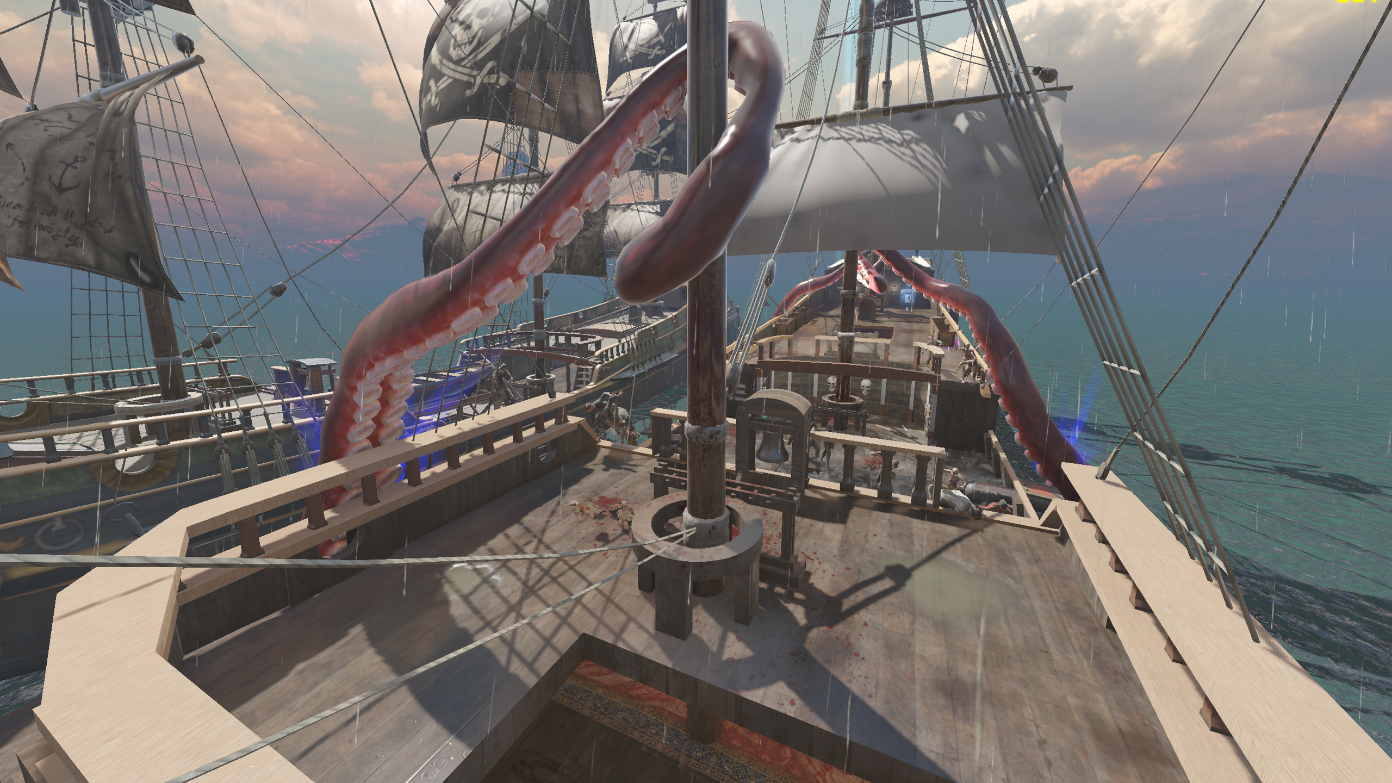
\includegraphics[width=\textwidth]{AAST.png}
    \caption{Bershama system architecture and reference design (first page image)}
    \label{fig:uml}
\end{figure}

\subsection{Core Components}

The system is built upon three foundational pillars:
\begin{enumerate}
    \item \textbf{Authenticated Shell:} \texttt{AuthenticatedShell} owns the header, navigation strip, console dock (admin surface), and user cluster. All authenticated pages render inside it; pages must not repeat chrome.
    \item \textbf{Surface Layouts:} Separate role-guarded layouts for \texttt{/admin}, \texttt{/pharmacy}, \texttt{/distributor}, \texttt{/driver}, and \texttt{/settings}.
    \item \textbf{Data Layer:} Supabase server clients (\texttt{createSupabaseServerClient} / \texttt{createSupabaseAdminClient}) with RLS; server actions under each feature folder (\texttt{products/actions.ts}, \texttt{requisitions/actions.ts}, \texttt{stocktake/actions.ts}, \texttt{alerts/actions.ts}, \texttt{deliveries/actions.ts}, \texttt{driver/actions.ts}).
\end{enumerate}

\subsection{User and Surface Hierarchies}

\begin{table}[h!]
    \centering
    \caption{User roles and authorized surfaces}
    \label{tab:roles}
    \begin{tabular}{lll}
        \hline
        \textbf{Role} & \textbf{Home Route} & \textbf{Authorized Surfaces} \\
        \hline
        Tenant Admin & \texttt{/admin} & Admin console \\
        Warehouse Manager / Dispatcher / Analyst & \texttt{/admin} & Admin console (read-only for Analyst) \\
        Pharmacy Manager & \texttt{/pharmacy} & Pharmacy orders only \\
        Driver & \texttt{/driver} & Driver run console only \\
        Distributor & \texttt{/distributor} & Distributor surface only \\
        \hline
    \end{tabular}
\end{table}

\section{Use Case: Authentication and Role-Based Routing}

The following scenario details the sign-in flow, illustrating the current defect and its required fix.

\subsection{Google Sign-In (Defect A1)}

\begin{enumerate}
    \item \textbf{Initiation:} User clicks ``Continue with Google'' on \texttt{/[locale]/login}. \texttt{components/google-signin-button.tsx} builds the OAuth redirect.
    \item \textbf{Current defect:} The redirect is always built as \texttt{?next=/\${locale}} regardless of where the user came from; \texttt{app/auth/callback/route.ts} exchanges the code and redirects to \texttt{safeNext} with no role lookup, so users land on the marketing landing page (\texttt{/en}) instead of their role home.
    \item \textbf{Required fix:} The button must accept a validated \texttt{next} deep link (defaulting to \texttt{/\${locale}}); after \texttt{exchangeCodeForSession}, the callback resolves the role via \texttt{getSession()} and redirects to \texttt{homeRouteForRole(role)}---TENANT\_ADMIN/WAREHOUSE\_MANAGER/DISPATCHER/ANALYST to \texttt{/admin}, DISTRIBUTOR to \texttt{/distributor}, PHARMACY\_MANAGER to \texttt{/pharmacy}, DRIVER to \texttt{/driver}---honoring a validated \texttt{next} when supplied.
    \item \textbf{Landing guard:} The public landing page must redirect already-signed-in visitors to their home route.
\end{enumerate}

\section{Remediation Plan (Pulled from GitHub)}

The full defect register and ordered fix tasks live in \texttt{docs/superpowers/plans/2026-10-29-bershama-remediation.md}. Summary of defect categories:

\subsection{A --- Auth / Redirect / Navigation}
\begin{itemize}
    \item \textbf{D1:} Google OAuth always lands on \texttt{/en}; no role resolution in callback.
    \item \textbf{D2:} auth.spec pharmacy/driver fail due to duplicate \texttt{<nav>} roles on rebuilt surfaces.
\end{itemize}

\subsection{B --- Duplicate Headers / Landmarks / Headings}
\begin{itemize}
    \item \textbf{D3:} Seven authenticated pages (\texttt{admin/alerts}, \texttt{admin/deliveries}, \texttt{admin/analytics}, \texttt{admin/inventory/stocktake}, \texttt{distributor}, \texttt{driver}, \texttt{pharmacy}) render their own \texttt{<header>} inside \texttt{AuthenticatedShell}.
    \item \textbf{D4:} Eight pages nest \texttt{<main>} inside the shell's \texttt{<main>}; most also use \texttt{min-h-[100dvh]}.
    \item \textbf{D5:} Duplicate \texttt{<h1>} in \texttt{components/signup-form.tsx} and \texttt{components/setup-form.tsx}.
\end{itemize}

\subsection{C --- Functionality Stripped by the Redesign}
\begin{itemize}
    \item \textbf{D6--D14:} Alerts (scan/ack/resolve), Deliveries (forms/map/run selection), Analytics (hardcoded chart, missing panels), Catalogue (inert search/filters, \texttt{?edit} ignored), Requisitions (allocate/release/approve/reject inert), Stocktake (empty count sheet), Pharmacy (dead \texttt{/admin/*} links, fake facility name), Driver (arrive/fail/signature/map gone), Distributor (dead \texttt{/admin/*} links, hardcoded badge).
\end{itemize}

\subsection{D --- Missing Routes and Dead Links}
\begin{itemize}
    \item \textbf{D15:} \texttt{/admin/audit} advertised but missing (404).
    \item \textbf{D16:} Distributor \texttt{routes} and Pharmacy \texttt{requisitions} nav items pending.
\end{itemize}

\subsection{E --- Layout / Typography}
\begin{itemize}
    \item \textbf{D17:} \texttt{xl:grid-cols4} typo to \texttt{xl:grid-cols-4}.
    \item \textbf{D18:} Invalid classes \texttt{font-body-md}, \texttt{font-body-sm}, \texttt{text-body-sm}, \texttt{font-cairo}.
    \item \textbf{D19:} \texttt{min-h-[100dvh]} inside page roots.
\end{itemize}

\subsection{F --- i18n / Copy}
\begin{itemize}
    \item \textbf{D20:} Namespace double-prefix bugs (\texttt{alerts.allClear} to \texttt{alerts.alerts.allClear}, \texttt{pharmacy.title} to \texttt{pharmacy.pharmacy.title}).
    \item \textbf{D21:} Hardcoded English strings in JSX.
\end{itemize}

\subsection{G --- Fake Data}
\begin{itemize}
    \item \textbf{D22:} Fabricated values presented as live: \texttt{Node 04}, \texttt{EGP 62,400}, \texttt{7e2f-90a1-c884}, \texttt{CAI-2026-N04}, \texttt{PH-1006}, fake pharmacies, fake proof rows, hardcoded chart axes.
\end{itemize}

\subsection{H --- Miscellaneous}
\begin{itemize}
    \item \textbf{D23:} Dead \texttt{href=\#} links.
    \item \textbf{D24:} Fake \texttt{bar-trend-chart} / \texttt{ranked-bars} testids on plain divs.
    \item \textbf{D25--D27:} E2E failures (5/36), hardcoded \texttt{/admin} redirects, untranslated dock labels.
\end{itemize}

\section{Verification and Acceptance Gates}

Before claiming completion, all of the following must pass:
\begin{enumerate}
    \item \texttt{make check}, \texttt{make typecheck}, \texttt{make lint}, \texttt{make build}, \texttt{make test} --- all green.
    \item \texttt{make e2e} --- 36/36 pass (alerts x3, auth pharmacy/driver fixed).
    \item One \texttt{<header>}, one \texttt{<main>}, one \texttt{<h1>} per authenticated page.
    \item \texttt{document.documentElement.scrollWidth <= innerWidth} at 1440 x 900, 834 x 1112, 390 x 844.
    \item Google sign-in lands on role home; \texttt{next} deep link honored.
    \item Grep for known fakes returns nothing.
    \item Lighthouse mobile + desktop documented in \texttt{docs/perf-2026-10-21.md}.
    \item Screenshots at 1440 x 900 / 834 x 1112 / 390 x 844, all pages, app vs design pairs in \texttt{/tmp/opencode/shots/\{design,app,pairs\}/}.
\end{enumerate}

\section{Out of Scope}

The Flutter mobile-app refactor is a scheduled job for a later phase and is not part of this submission.

\end{document}
